% Options for packages loaded elsewhere
\PassOptionsToPackage{unicode}{hyperref}
\PassOptionsToPackage{hyphens}{url}
\PassOptionsToPackage{dvipsnames,svgnames,x11names}{xcolor}
%
\documentclass[
  letterpaper,
  DIV=11,
  numbers=noendperiod]{scrreprt}

\usepackage{amsmath,amssymb}
\usepackage{lmodern}
\usepackage{iftex}
\ifPDFTeX
  \usepackage[T1]{fontenc}
  \usepackage[utf8]{inputenc}
  \usepackage{textcomp} % provide euro and other symbols
\else % if luatex or xetex
  \usepackage{unicode-math}
  \defaultfontfeatures{Scale=MatchLowercase}
  \defaultfontfeatures[\rmfamily]{Ligatures=TeX,Scale=1}
\fi
% Use upquote if available, for straight quotes in verbatim environments
\IfFileExists{upquote.sty}{\usepackage{upquote}}{}
\IfFileExists{microtype.sty}{% use microtype if available
  \usepackage[]{microtype}
  \UseMicrotypeSet[protrusion]{basicmath} % disable protrusion for tt fonts
}{}
\makeatletter
\@ifundefined{KOMAClassName}{% if non-KOMA class
  \IfFileExists{parskip.sty}{%
    \usepackage{parskip}
  }{% else
    \setlength{\parindent}{0pt}
    \setlength{\parskip}{6pt plus 2pt minus 1pt}}
}{% if KOMA class
  \KOMAoptions{parskip=half}}
\makeatother
\usepackage{xcolor}
\setlength{\emergencystretch}{3em} % prevent overfull lines
\setcounter{secnumdepth}{5}
% Make \paragraph and \subparagraph free-standing
\ifx\paragraph\undefined\else
  \let\oldparagraph\paragraph
  \renewcommand{\paragraph}[1]{\oldparagraph{#1}\mbox{}}
\fi
\ifx\subparagraph\undefined\else
  \let\oldsubparagraph\subparagraph
  \renewcommand{\subparagraph}[1]{\oldsubparagraph{#1}\mbox{}}
\fi

\usepackage{color}
\usepackage{fancyvrb}
\newcommand{\VerbBar}{|}
\newcommand{\VERB}{\Verb[commandchars=\\\{\}]}
\DefineVerbatimEnvironment{Highlighting}{Verbatim}{commandchars=\\\{\}}
% Add ',fontsize=\small' for more characters per line
\usepackage{framed}
\definecolor{shadecolor}{RGB}{248,248,248}
\newenvironment{Shaded}{\begin{snugshade}}{\end{snugshade}}
\newcommand{\AlertTok}[1]{\textcolor[rgb]{0.94,0.16,0.16}{#1}}
\newcommand{\AnnotationTok}[1]{\textcolor[rgb]{0.56,0.35,0.01}{\textbf{\textit{#1}}}}
\newcommand{\AttributeTok}[1]{\textcolor[rgb]{0.77,0.63,0.00}{#1}}
\newcommand{\BaseNTok}[1]{\textcolor[rgb]{0.00,0.00,0.81}{#1}}
\newcommand{\BuiltInTok}[1]{#1}
\newcommand{\CharTok}[1]{\textcolor[rgb]{0.31,0.60,0.02}{#1}}
\newcommand{\CommentTok}[1]{\textcolor[rgb]{0.56,0.35,0.01}{\textit{#1}}}
\newcommand{\CommentVarTok}[1]{\textcolor[rgb]{0.56,0.35,0.01}{\textbf{\textit{#1}}}}
\newcommand{\ConstantTok}[1]{\textcolor[rgb]{0.00,0.00,0.00}{#1}}
\newcommand{\ControlFlowTok}[1]{\textcolor[rgb]{0.13,0.29,0.53}{\textbf{#1}}}
\newcommand{\DataTypeTok}[1]{\textcolor[rgb]{0.13,0.29,0.53}{#1}}
\newcommand{\DecValTok}[1]{\textcolor[rgb]{0.00,0.00,0.81}{#1}}
\newcommand{\DocumentationTok}[1]{\textcolor[rgb]{0.56,0.35,0.01}{\textbf{\textit{#1}}}}
\newcommand{\ErrorTok}[1]{\textcolor[rgb]{0.64,0.00,0.00}{\textbf{#1}}}
\newcommand{\ExtensionTok}[1]{#1}
\newcommand{\FloatTok}[1]{\textcolor[rgb]{0.00,0.00,0.81}{#1}}
\newcommand{\FunctionTok}[1]{\textcolor[rgb]{0.00,0.00,0.00}{#1}}
\newcommand{\ImportTok}[1]{#1}
\newcommand{\InformationTok}[1]{\textcolor[rgb]{0.56,0.35,0.01}{\textbf{\textit{#1}}}}
\newcommand{\KeywordTok}[1]{\textcolor[rgb]{0.13,0.29,0.53}{\textbf{#1}}}
\newcommand{\NormalTok}[1]{#1}
\newcommand{\OperatorTok}[1]{\textcolor[rgb]{0.81,0.36,0.00}{\textbf{#1}}}
\newcommand{\OtherTok}[1]{\textcolor[rgb]{0.56,0.35,0.01}{#1}}
\newcommand{\PreprocessorTok}[1]{\textcolor[rgb]{0.56,0.35,0.01}{\textit{#1}}}
\newcommand{\RegionMarkerTok}[1]{#1}
\newcommand{\SpecialCharTok}[1]{\textcolor[rgb]{0.00,0.00,0.00}{#1}}
\newcommand{\SpecialStringTok}[1]{\textcolor[rgb]{0.31,0.60,0.02}{#1}}
\newcommand{\StringTok}[1]{\textcolor[rgb]{0.31,0.60,0.02}{#1}}
\newcommand{\VariableTok}[1]{\textcolor[rgb]{0.00,0.00,0.00}{#1}}
\newcommand{\VerbatimStringTok}[1]{\textcolor[rgb]{0.31,0.60,0.02}{#1}}
\newcommand{\WarningTok}[1]{\textcolor[rgb]{0.56,0.35,0.01}{\textbf{\textit{#1}}}}

\providecommand{\tightlist}{%
  \setlength{\itemsep}{0pt}\setlength{\parskip}{0pt}}\usepackage{longtable,booktabs,array}
\usepackage{calc} % for calculating minipage widths
% Correct order of tables after \paragraph or \subparagraph
\usepackage{etoolbox}
\makeatletter
\patchcmd\longtable{\par}{\if@noskipsec\mbox{}\fi\par}{}{}
\makeatother
% Allow footnotes in longtable head/foot
\IfFileExists{footnotehyper.sty}{\usepackage{footnotehyper}}{\usepackage{footnote}}
\makesavenoteenv{longtable}
\usepackage{graphicx}
\makeatletter
\def\maxwidth{\ifdim\Gin@nat@width>\linewidth\linewidth\else\Gin@nat@width\fi}
\def\maxheight{\ifdim\Gin@nat@height>\textheight\textheight\else\Gin@nat@height\fi}
\makeatother
% Scale images if necessary, so that they will not overflow the page
% margins by default, and it is still possible to overwrite the defaults
% using explicit options in \includegraphics[width, height, ...]{}
\setkeys{Gin}{width=\maxwidth,height=\maxheight,keepaspectratio}
% Set default figure placement to htbp
\makeatletter
\def\fps@figure{htbp}
\makeatother
\newlength{\cslhangindent}
\setlength{\cslhangindent}{1.5em}
\newlength{\csllabelwidth}
\setlength{\csllabelwidth}{3em}
\newlength{\cslentryspacingunit} % times entry-spacing
\setlength{\cslentryspacingunit}{\parskip}
\newenvironment{CSLReferences}[2] % #1 hanging-ident, #2 entry spacing
 {% don't indent paragraphs
  \setlength{\parindent}{0pt}
  % turn on hanging indent if param 1 is 1
  \ifodd #1
  \let\oldpar\par
  \def\par{\hangindent=\cslhangindent\oldpar}
  \fi
  % set entry spacing
  \setlength{\parskip}{#2\cslentryspacingunit}
 }%
 {}
\usepackage{calc}
\newcommand{\CSLBlock}[1]{#1\hfill\break}
\newcommand{\CSLLeftMargin}[1]{\parbox[t]{\csllabelwidth}{#1}}
\newcommand{\CSLRightInline}[1]{\parbox[t]{\linewidth - \csllabelwidth}{#1}\break}
\newcommand{\CSLIndent}[1]{\hspace{\cslhangindent}#1}

\usepackage{fontspec}
\usepackage{polyglossia}
\setmonofont{JuliaMono}[Scale=MatchLowercase]
\usepackage{latexsym,exscale,stmaryrd,amsmath,amssymb}
\usepackage{unicode-math}
\newcommand{\uu}[1]{{\mathbf{\boldsymbol{{#1}}}}}
\newcommand{\uuuu}[1]{{\mathbb{{#1}}}}
\newcommand{\uv}[1]{{\underline{{#1}}}}
\newcommand{\trans}[1]{{{}^{t}{#1}}}
\newcommand{\sotimes}{{\stackrel{s}{\otimes}}}
\newcommand{\norm}[1]{{\lVert{{#1}}\rVert}}
\newcommand{\ud}{{\,\mathrm{d}}}
\DeclareMathOperator{\arcosh}{arcosh}
\KOMAoption{captions}{tableheading}
\makeatletter
\makeatother
\makeatletter
\@ifpackageloaded{bookmark}{}{\usepackage{bookmark}}
\makeatother
\makeatletter
\@ifpackageloaded{caption}{}{\usepackage{caption}}
\AtBeginDocument{%
\ifdefined\contentsname
  \renewcommand*\contentsname{Table of contents}
\else
  \newcommand\contentsname{Table of contents}
\fi
\ifdefined\listfigurename
  \renewcommand*\listfigurename{List of Figures}
\else
  \newcommand\listfigurename{List of Figures}
\fi
\ifdefined\listtablename
  \renewcommand*\listtablename{List of Tables}
\else
  \newcommand\listtablename{List of Tables}
\fi
\ifdefined\figurename
  \renewcommand*\figurename{Figure}
\else
  \newcommand\figurename{Figure}
\fi
\ifdefined\tablename
  \renewcommand*\tablename{Table}
\else
  \newcommand\tablename{Table}
\fi
}
\@ifpackageloaded{float}{}{\usepackage{float}}
\floatstyle{ruled}
\@ifundefined{c@chapter}{\newfloat{codelisting}{h}{lop}}{\newfloat{codelisting}{h}{lop}[chapter]}
\floatname{codelisting}{Listing}
\newcommand*\listoflistings{\listof{codelisting}{List of Listings}}
\makeatother
\makeatletter
\@ifpackageloaded{caption}{}{\usepackage{caption}}
\@ifpackageloaded{subcaption}{}{\usepackage{subcaption}}
\makeatother
\makeatletter
\makeatother
\ifLuaTeX
  \usepackage{selnolig}  % disable illegal ligatures
\fi
\IfFileExists{bookmark.sty}{\usepackage{bookmark}}{\usepackage{hyperref}}
\IfFileExists{xurl.sty}{\usepackage{xurl}}{} % add URL line breaks if available
\urlstyle{same} % disable monospaced font for URLs
\hypersetup{
  pdftitle={ECHOES},
  pdfauthor={Jean-François Barthélémy},
  colorlinks=true,
  linkcolor={blue},
  filecolor={Maroon},
  citecolor={Blue},
  urlcolor={Blue},
  pdfcreator={LaTeX via pandoc}}

\title{ECHOES}
\usepackage{etoolbox}
\makeatletter
\providecommand{\subtitle}[1]{% add subtitle to \maketitle
  \apptocmd{\@title}{\par {\large #1 \par}}{}{}
}
\makeatother
\subtitle{Extended Calculator of HOmogEnization Schemes}
\author{Jean-François Barthélémy}
\date{10/22/22}

\begin{document}
\maketitle
\renewcommand*\contentsname{Table of contents}
{
\hypersetup{linkcolor=}
\setcounter{tocdepth}{2}
\tableofcontents
}
\bookmarksetup{startatroot}

\hypertarget{welcome}{%
\chapter*{Welcome}\label{welcome}}
\addcontentsline{toc}{chapter}{Welcome}

\markboth{Welcome}{Welcome}

This manual aims at recalling some fundamental aspects of the theory of
homogenization of random media along with a presentation of the main
features of the library \textbf{ECHOES} as well as code examples.

The library \textbf{ECHOES} allows to implement various homogenization
schemes involving different types of heterogeneities in the framework of
elasticity, conductivity, viscoelasticity as well as tools to properly
calculate the derivatives of macroscopic stiffness with respect to lower
scale moduli (fundamental tool of the modified secant method in
nonlinear homogenization).

\bookmarksetup{startatroot}

\hypertarget{introduction}{%
\chapter{Introduction}\label{introduction}}

\bookmarksetup{startatroot}

\hypertarget{summary}{%
\chapter{Summary}\label{summary}}

In summary, this book has no content whatsoever.

\bookmarksetup{startatroot}

\hypertarget{references}{%
\chapter*{References}\label{references}}
\addcontentsline{toc}{chapter}{References}

\markboth{References}{References}

\hypertarget{refs}{}
\begin{CSLReferences}{1}{0}
\leavevmode\vadjust pre{\hypertarget{ref-abramowitz1972}{}}%
Abramowitz, M., Stegun, I.A., 1972. Handbook of {Mathematical
Functions}. {National Bureau of Standards - Applied Mathematics Series -
55}, {Washington D.C.}

\leavevmode\vadjust pre{\hypertarget{ref-barthelemy2020}{}}%
Barthélémy, J.-F., 2020. Simplified approach to the derivation of the
relationship between {Hill} polarization tensors of transformed problems
and applications. International Journal of Engineering Science 154,
103326. \url{https://doi.org/10.1016/j.ijengsci.2020.103326}

\leavevmode\vadjust pre{\hypertarget{ref-barthelemy2009c}{}}%
Barthélémy, J.-F., 2009. Compliance and {Hill} polarization tensor of a
crack in an anisotropic matrix. International Journal of Solids and
Structures 46, 4064--4072.
\url{https://doi.org/10.1016/j.ijsolstr.2009.08.003}

\leavevmode\vadjust pre{\hypertarget{ref-barthelemy2021}{}}%
Barthélémy, J.-F., Sevostianov, I., Giraud, A., 2021. Micromechanical
modeling of a cracked elliptically orthotropic medium. International
Journal of Engineering Science 161, 103454.
\url{https://doi.org/10.1016/j.ijengsci.2021.103454}

\leavevmode\vadjust pre{\hypertarget{ref-eshelby1957}{}}%
Eshelby, J.D., 1957. The determination of the elastic field of an
ellipsoidal inclusion, and related problems. Proceedings of the Royal
Society of London. Series A. Mathematical and Physical Sciences 241,
376--396. \url{https://doi.org/10.1098/rspa.1957.0133}

\leavevmode\vadjust pre{\hypertarget{ref-gavazzi1990}{}}%
Gavazzi, A.C., Lagoudas, D.C., 1990. On the numerical evaluation of
{Eshelby}'s tensor and its application to elastoplastic fibrous
composites. Computational Mechanics 7, 13--19.
\url{https://doi.org/10.1007/BF00370053}

\leavevmode\vadjust pre{\hypertarget{ref-ghahremani1977}{}}%
Ghahremani, F., 1977. Numerical evaluation of the stresses and strains
in ellipsoidal inclusions in an anisotropic elastic material. Mechanics
Research Communications 4, 89--91.
\url{https://doi.org/10.1016/0093-6413(77)90018-0}

\leavevmode\vadjust pre{\hypertarget{ref-kellogg1929}{}}%
Kellogg, O.D., 1929. Potential theory. {Berlin : Springer-Verlag}.

\leavevmode\vadjust pre{\hypertarget{ref-masson2008}{}}%
Masson, R., 2008. New explicit expressions of the {Hill} polarization
tensor for general anisotropic elastic solids. International Journal of
Solids and Structures 45, 757--769.
\url{https://doi.org/10.1016/j.ijsolstr.2007.08.035}

\leavevmode\vadjust pre{\hypertarget{ref-mura1987}{}}%
Mura, T., 1987. Micromechanics of {Defects} in {Solids}, {Second
Edition}. {Kluwer Academic}.
\url{https://doi.org/10.1002/zamm.19890690204}

\leavevmode\vadjust pre{\hypertarget{ref-willis1977}{}}%
Willis, J.R., 1977. Bounds and self-consistent estimates for the overall
properties of anisotropic composites. Journal of the Mechanics and
Physics of Solids 25, 185--202.
\url{https://doi.org/10.1016/0022-5096(77)90022-9}

\leavevmode\vadjust pre{\hypertarget{ref-withers1989}{}}%
Withers, P.J., 1989. The determination of the elastic field of an
ellipsoidal inclusion in a transversely isotropic medium, and its
relevance to composite materials. Philosophical Magazine A 59, 759--781.
\url{https://doi.org/10.1080/01418618908209819}

\end{CSLReferences}

\appendix
\addcontentsline{toc}{part}{Appendices}

\hypertarget{hill-polarization-tensor}{%
\chapter{Hill polarization tensor}\label{hill-polarization-tensor}}

This section recalls some results about the calculation of the Hill
polarization tensors related to a matrix of stiffness \(\mathbb{C}\) and
an ellipsoid \(\mathcal{E}_{{\mathbf{\boldsymbol{{A}}}}}\) of equation
\[
{\underline{{x}}}\in\mathcal{E}_{{\mathbf{\boldsymbol{{A}}}}}
\quad\Leftrightarrow\quad
{\underline{{x}}}\cdot({{}^{t}{{\mathbf{\boldsymbol{{A}}}}}}\cdot{\mathbf{\boldsymbol{{A}}}})^{-1}\cdot{\underline{{x}}}\leq 1
\] where \({\mathbf{\boldsymbol{{A}}}}\) is an invertible second-order
tensor so that
\({{}^{t}{{\mathbf{\boldsymbol{{A}}}}}}\cdot{\mathbf{\boldsymbol{{A}}}}\)
is a positive definite symmetric tensor associated to 3 radii
(eigenvalues \(a\geq b \geq c\) possibly written
\(\rho_1 \geq \rho_2 \geq \rho_3\) for convenience) and 3 angles
(orientation of the frame of eigenvectors
\({\underline{{e}}}_1, {\underline{{e}}}_2, {\underline{{e}}}_3\))
\begin{equation}\protect\hypertarget{eq-ellipsoid}{}{
{{}^{t}{{\mathbf{\boldsymbol{{A}}}}}}\cdot{\mathbf{\boldsymbol{{A}}}}=a^2 {\underline{{e}}}_1\otimes{\underline{{e}}}_1 + b^2 {\underline{{e}}}_2\otimes{\underline{{e}}}_2 + c^2 {\underline{{e}}}_3\otimes{\underline{{e}}}_3 = \sum_{i=1}^3 \rho_i {\underline{{e}}}_i\otimes{\underline{{e}}}_i
}\label{eq-ellipsoid}\end{equation}

\hypertarget{general-expression}{%
\section{General expression}\label{general-expression}}

A general expression of the elastic polarization tensor is derived in
(\protect\hyperlink{ref-willis1977}{Willis, 1977}) (see also
(\protect\hyperlink{ref-mura1987}{Mura, 1987}))
\begin{equation}\protect\hypertarget{eq-Hill}{}{\begin{aligned}
{\mathbb{{P}}}({\mathbf{\boldsymbol{{A}}}},{\mathbb{{C}}})&=\frac{1}{4\pi}
\int_{{\lVert{{{\underline{{\zeta}}}}}\rVert}=1}
({\mathbf{\boldsymbol{{A}}}}^{-1}\cdot{\underline{{\zeta}}}){\stackrel{s}{\otimes}}
\Big(({\mathbf{\boldsymbol{{A}}}}^{-1}\cdot{\underline{{\zeta}}})\cdot{\mathbb{{C}}}
\cdot({\mathbf{\boldsymbol{{A}}}}^{-1}\cdot{\underline{{\zeta}}})\Big)^{-1}
{\stackrel{s}{\otimes}}({\mathbf{\boldsymbol{{A}}}}^{-1}\cdot{\underline{{\zeta}}})
{\,\mathrm{d}}S_\zeta\\
&=
\frac{\det{{\mathbf{\boldsymbol{{A}}}}}}{4\pi}
\int_{{\lVert{{{\underline{{\xi}}}}}\rVert}=1}
\frac{{\underline{{\xi}}}{\stackrel{s}{\otimes}}
({\underline{{\xi}}}\cdot{\mathbb{{C}}}
\cdot{\underline{{\xi}}})^{-1}
{\stackrel{s}{\otimes}}{\underline{{\xi}}}}{{\lVert{{{\mathbf{\boldsymbol{{A}}}}\cdot{\underline{{\xi}}}}}\rVert}^3}
{\,\mathrm{d}}S_{\xi}
\end{aligned}}\label{eq-Hill}\end{equation}

When \({\mathbb{{C}}}\) is arbitrarily anisotropic, it is necessary to
resort to numerical cubature to estimate \({\mathbb{{P}}}\) as proposed
in (\protect\hyperlink{ref-ghahremani1977}{Ghahremani, 1977}),
(\protect\hyperlink{ref-gavazzi1990}{Gavazzi and Lagoudas, 1990}) or
(\protect\hyperlink{ref-masson2008}{Masson, 2008}). However in some
cases of anisotropy, analytical solutions are available
((\protect\hyperlink{ref-withers1989}{Withers, 1989}),
(\protect\hyperlink{ref-barthelemy2020}{Barthélémy, 2020})). The case of
isotropic matrix is particularly developed in the next section.

\hypertarget{isotropic-matrix}{%
\section{Isotropic matrix}\label{isotropic-matrix}}

In this section, the matrix is assumed isotropic so that its stiffness
tensor writes by means of a bulk \(k\) and shear \(\mu\) or Lamé
\(\lambda\) and \(\mu\) moduli or even Young modulus \(E\) and Poisson
ratio \(\nu\) with \(k=\frac{E}{3(1-2\nu)}\) and
\(\mu=\frac{E}{2(1+\nu)}\).
\begin{equation}\protect\hypertarget{eq-isoC}{}{\begin{aligned}
{\mathbb{{C}}} =& {} 3k{\mathbb{{J}}}+2\mu{\mathbb{{K}}} =  3\lambda{\mathbb{{I}}}+2\mu{\mathbb{{K}}}\\
 & \quad\textrm{with}\quad J_{ijkl}=\frac{\delta_{ij}\delta_{kl}}{3},
I_{ijkl}=\frac{\delta_{ik}\delta_{jl}+\delta_{il}\delta_{jk}}{2}
\textrm{ and }
{\mathbb{{K}}}={\mathbb{{I}}}-{\mathbb{{J}}}
\end{aligned}}\label{eq-isoC}\end{equation}

Introducing Equation~\ref{eq-isoC} in Equation~\ref{eq-Hill} leads to
after some algebra \[
{\mathbb{{P}}}=
\frac{1}{\lambda+2\,\mu}
{\mathbb{{U}}}
+\frac{1}{\mu}({\mathbb{{V}}}-{\mathbb{{U}}})
\] where the tensors \({\mathbb{{U}}}\) and \({\mathbb{{V}}}\),
depending only on the ellipsoidal tensor \({\mathbf{\boldsymbol{{A}}}}\)
of Equation~\ref{eq-ellipsoid}, are given by (see
(\protect\hyperlink{ref-barthelemy2020}{Barthélémy, 2020}))
\[\begin{aligned}
{\mathbb{{U}}} &= \frac{\det{{\mathbf{\boldsymbol{{A}}}}}}{4\pi}
\int_{{\lVert{{{\underline{{\xi}}}}}\rVert}=1}
\frac{{\underline{{\xi}}}\otimes{\underline{{\xi}}}\otimes{\underline{{\xi}}}\otimes{\underline{{\xi}}}}
{{\lVert{{{\mathbf{\boldsymbol{{A}}}}\cdot{\underline{{\xi}}}}}\rVert}^3}{\,\mathrm{d}}S_{\xi}\\
&=
\frac{1}{4\pi}
\int_{{\lVert{{{\underline{{\zeta}}}}}\rVert}=1}
\frac{%
({\mathbf{\boldsymbol{{A}}}}^{-1}\cdot{\underline{{\zeta}}})
\otimes
({\mathbf{\boldsymbol{{A}}}}^{-1}\cdot{\underline{{\zeta}}})
\otimes
({\mathbf{\boldsymbol{{A}}}}^{-1}\cdot{\underline{{\zeta}}})
\otimes
({\mathbf{\boldsymbol{{A}}}}^{-1}\cdot{\underline{{\zeta}}})
}{{\lVert{{{\mathbf{\boldsymbol{{A}}}}^{-1}\cdot{\underline{{\zeta}}}}}\rVert}^4}
{\,\mathrm{d}}S_{\zeta}
\end{aligned}\] and \[\begin{aligned}
{\mathbb{{V}}} &= \frac{\det{{\mathbf{\boldsymbol{{A}}}}}}{4\pi}
\int_{{\lVert{{{\underline{{\xi}}}}}\rVert}=1}
\frac{{\underline{{\xi}}}{\stackrel{s}{\otimes}}{\mathbf{\boldsymbol{{1}}}}{\stackrel{s}{\otimes}}{\underline{{\xi}}}}
{{\lVert{{{\mathbf{\boldsymbol{{A}}}}\cdot{\underline{{\xi}}}}}\rVert}^3}{\,\mathrm{d}}S_{\xi}\\
&=
\frac{1}{4\pi}
\int_{{\lVert{{{\underline{{\zeta}}}}}\rVert}=1}
\frac{%
({\mathbf{\boldsymbol{{A}}}}^{-1}\cdot{\underline{{\zeta}}})
{\stackrel{s}{\otimes}}
{\mathbf{\boldsymbol{{1}}}}
{\stackrel{s}{\otimes}}
({\mathbf{\boldsymbol{{A}}}}^{-1}\cdot{\underline{{\zeta}}})
}{{\lVert{{{\mathbf{\boldsymbol{{A}}}}^{-1}\cdot{\underline{{\zeta}}}}}\rVert}^2}
{\,\mathrm{d}}S_{\zeta}
\end{aligned}\] For an arbitrary ellipsoid defined by
Equation~\ref{eq-ellipsoid}, the components of \({\mathbb{{U}}}\) and
\({\mathbb{{V}}}\) write \[\begin{aligned}
U_{iiii}&=\frac{3(I_i-\rho_i^2I_{ii})}{2} 
\quad\forall\, i\in\{1,2,3\}\\
U_{iijj}=U_{ijij}=U_{ijji}&=\frac{I_j-\rho_i^2I_{ij}}{2} 
=\frac{I_i-\rho_j^2I_{ij}}{2}
\quad\forall\, i\neq j\in\{1,2,3\}
\end{aligned}\] and \[\begin{aligned}
V_{iiii}&=I_i\quad\forall\, i\in\{1,2,3\}\\
V_{ijij}=V_{ijji}&=\frac{I_i+I_j}{4}
\quad\forall\, i\neq j\in\{1,2,3\}
\end{aligned}\] where the coefficients \(I_i\) and \(I_{ij}\) are given
by (note that \(I_i\) and \(I_{ij}\) are adapted from those provided in
(\protect\hyperlink{ref-kellogg1929}{Kellogg, 1929}) and
(\protect\hyperlink{ref-eshelby1957}{Eshelby, 1957}): they differ by a
factor of \(4\pi/3\) for \(I_{ij}\) with \(i\neq j\) and by \(4\pi\) for
the others)

\begin{itemize}
\tightlist
\item
  if \(a > b > c\) \[\begin{aligned}
    I_1&=\frac{a\,b\,c}{(a^2-b^2)\sqrt{a^2-c^2}}\,
    \left({\cal F}-{\cal E}\right)\\
    I_3&=\frac{a\,b\,c}{(b^2-c^2)\sqrt{a^2-c^2}}\,
    \left(\frac{b\sqrt{a^2-c^2}}{a\,c}-
    {\cal E}\right)\\
    I_2&=1-I_1-I_3\\
    I_{ij}&=\frac{I_j-I_i}{\rho_i^2-\rho_j^2}\quad\forall\, i\neq j\in\{1,2,3\}\\
    I_{ii}&=\frac{1}{3}\left(
    \frac{1}{\rho_i^2}-
    \sum_{j\neq i}I_{ij} \right) 
    \quad\forall\, i\in\{1,2,3\}
    \end{aligned}\]\\
  where \({\cal F}={\cal F}(\theta,\kappa)\) and
  \({\cal E}={\cal E}(\theta,\kappa)\) are respectively the elliptic
  integrals of the first and second kinds (see
  (\protect\hyperlink{ref-abramowitz1972}{Abramowitz and Stegun, 1972}))
  of amplitude and parameter \[
    \theta=\arcsin{\sqrt{1-\frac{c^2}{a^2}}}
    \quad;\quad
    \kappa=\sqrt{\frac{a^2-b^2}{a^2-c^2}}
    \]
\item
  if \(a > b = c\) (prolate spheroid) \[\begin{aligned}
    I_2=I_3&=a\,
    \frac{a\sqrt{a^2-c^2}-c^2\,\mathop{\mathrm{arcosh}}{(a/c)}}
    {2\left(a^2-c^2\right)^{3/2}}\\
    I_1&=1-2\,I_3\\
    I_{1i}=I_{i1}&=\frac{I_i-I_1}{a^2-\rho_i^2}\quad
    \forall\, i\in\{2,3\}\\
    I_{ij}&=\frac{1}{4}
    \left(\frac{1}{c^2}-I_{31} \right) 
    \quad\forall\, i,j\in\{2,3\}\\
    I_{11}&=\frac{1}{3}
    \left(\frac{1}{a^2}-2\,I_{31} \right)
    \end{aligned}\]
\item
  if \(a = b > c\) (oblate spheroid) \[\begin{aligned}
    I_1=I_2&=c\,
    \frac{a^2\,\arccos{(c/a)}-c\sqrt{a^2-c^2}}
    {2\left(a^2-c^2\right)^{3/2}}\\
    I_3&=1-2\,I_1\\
    I_{3i}=I_{i3}&=\frac{I_3-I_i}{\rho_i^2-c^2}\quad
    \forall\, i\in\{1,2\}\\
    I_{ij}&=\frac{1}{4}
    \left(\frac{1}{a^2}-I_{31} \right) 
    \quad\forall\, i,j\in\{1,2\}\\
    I_{33}&=\frac{1}{3}
    \left(\frac{1}{c^2}-2\,I_{31} \right)
    \end{aligned}\]
\item
  if \(a = b = c\) (sphere) \[\begin{aligned}
    I_1=I_2=I_3&=\frac{1}{3}\\
    I_{ij}&=\frac{1}{5\,a^2}\quad\forall\, i,j\in\{1,2,3\}
    \end{aligned}\]
\end{itemize}

In this last case of spherical inclusion
(\({\mathbf{\boldsymbol{{A}}}}={\mathbf{\boldsymbol{{1}}}}\)),
\({\mathbb{{U}}}\) and \({\mathbb{{V}}}\) are simply decomposed as \[
{\mathbb{{U}}}=\frac{1}{3}{\mathbb{{J}}}+\frac{2}{15}{\mathbb{{K}}}
\quad\textrm{ and }\quad
{\mathbb{{V}}}=\frac{1}{3}{\mathbb{{I}}}
\]

\hypertarget{case-of-cracks}{%
\section{Case of cracks}\label{case-of-cracks}}

The case of cracks corresponds to ellipsoids for which the smallest
radius is very small compared to the two others, in other words the
characteristic tensor \({\mathbf{\boldsymbol{{A}}}}\)
Equation~\ref{eq-ellipsoid} can be written here \[
{\mathbf{\boldsymbol{{A}}}}=
{\underline{{\ell}}}\otimes{\underline{{\ell}}}+
\eta\,{\underline{{m}}}\otimes{\underline{{m}}}+
\omega\,{\underline{{n}}}\otimes{\underline{{n}}}
\quad\textrm{with}\quad
\eta=\frac{b}{a}
\quad\textrm{and}\quad
\omega=\frac{c}{a}
\]

\begin{figure}

{\centering 

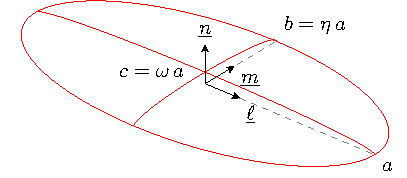
\includegraphics[width=0.5\textwidth,height=\textheight]{./images/ellipsoidalcrack.pdf}

}

\caption{\label{fig-crack}Ellipsoidal crack}

\end{figure}

In the case of cracks, it is useful to introduce the second Hill
polarization tensor defined as \[
{\mathbb{{Q}}}={\mathbb{{C}}}-{\mathbb{{C}}}:{\mathbb{{P}}}:{\mathbb{{C}}}
\] and in particular \(\lim_{\omega\to 0}\omega\,{\mathbb{{Q}}}^{-1}\)
in which it is recalled that \({\mathbb{{P}}}\) and thus
\({\mathbb{{Q}}}\) depend on \(\omega\) such that the components
\(Q_{nijk}\) (with \(n\) corresponding to the crack normal) behave as
\(1/\omega\) when \(\omega\) tends towards \(0\). The analytical
expressions of this limit are fully detailed in
(\protect\hyperlink{ref-barthelemy2021}{Barthélémy et al., 2021}) which
recalls in particular that \({\mathbb{{L}}}\) actually derives from a
symmetric second-order tensor \({\mathbf{\boldsymbol{{B}}}}\) as
\begin{equation}\protect\hypertarget{eq-L}{}{
{\mathbb{{L}}}=
\lim_{\omega\to 0} \omega\,{\mathbb{{Q}}}^{-1}
=\frac{3}{4}\,{\underline{{n}}}{\stackrel{s}{\otimes}}{\mathbf{\boldsymbol{{B}}}}{\stackrel{s}{\otimes}}{\underline{{n}}}
}\label{eq-L}\end{equation}

For an arbitrarly anisotropic matrix, an algorithm allowing to estimate
the limit Equation~\ref{eq-L} is proposed in
(\protect\hyperlink{ref-barthelemy2009c}{Barthélémy, 2009}) whereas in
the isotropic case \({\mathbf{\boldsymbol{{B}}}}\) writes \[
{\mathbf{\boldsymbol{{B}}}}=
B_{nn}\,{\underline{{n}}}\otimes{\underline{{n}}}
+
B_{mm}\,{\underline{{m}}}\otimes{\underline{{m}}}
+
B_{\ell\ell}\,{\underline{{\ell}}}\otimes{\underline{{\ell}}}
\] with \[\begin{aligned}
B_{nn}&=\frac{8\,\eta\,(1-\nu^2)}{3\,E}\,
\frac{1}{\mathcal{E}_\eta}\label{eq:Bnn}\\
B_{mm}&=\frac{8\,\eta\,(1-\nu^2)}{3\,E}\,
\frac{1-\eta^2}{\left(1-(1-\nu)\,\eta^2\right)
\,\mathcal{E}_\eta-\nu\,\eta^2\,\mathcal{K}_\eta}\\
B_{\ell\ell}&=\frac{8\,\eta\,(1-\nu^2)}{3\,E}\,
\frac{1-\eta^2}{(1-\nu-\eta^2)\,\mathcal{E}_\eta+\nu\,\eta^2\,\mathcal{K}_\eta}
\end{aligned}\] where \(\mathcal{K}_\eta=\mathcal{K}(\sqrt{1-\eta^2})\)
and \(\mathcal{E}_\eta=\mathcal{E}(\sqrt{1-\eta^2})\) are the complete
elliptic integrals of respectively the first and second kind (see
(\protect\hyperlink{ref-abramowitz1972}{Abramowitz and Stegun, 1972})).
If the crack is circular, the components of
\({\mathbf{\boldsymbol{{B}}}}\) become \[
B_{nn}=\frac{16\,(1-\nu^2)}{3\,\pi\,E}
\quad\textrm{;}\quad
B_{mm}=B_{\ell\ell}=\frac{B_{nn}}{1-\nu/2}
\]

\hypertarget{application-of-hill-calculation}{%
\section{Application of Hill
calculation}\label{application-of-hill-calculation}}

\begin{Shaded}
\begin{Highlighting}[]
\ImportTok{import}\NormalTok{ numpy }\ImportTok{as}\NormalTok{ np}
\ImportTok{from}\NormalTok{ echoes }\ImportTok{import} \OperatorTok{*}
\ImportTok{import}\NormalTok{ matplotlib.pyplot }\ImportTok{as}\NormalTok{ plt}
\end{Highlighting}
\end{Shaded}

\begin{verbatim}
RuntimeError: FATAL: module compiled as little endian, but detected different endianness at runtime
\end{verbatim}

\hypertarget{definition-of-the-matrix-tensor}{%
\subsection{Definition of the matrix
tensor}\label{definition-of-the-matrix-tensor}}

\begin{Shaded}
\begin{Highlighting}[]
\NormalTok{C }\OperatorTok{=}\NormalTok{ stiff\_Enu(}\FloatTok{1.}\NormalTok{,}\FloatTok{0.2}\NormalTok{) }\OperatorTok{;} \BuiltInTok{print}\NormalTok{(C)}
\end{Highlighting}
\end{Shaded}

\begin{verbatim}
Order 4 ISO tensor | Param(size=2)=[ 1.66667 0.833333 ] | Angles(size=0)=[ ]
[ 1.11111 0.277778 0.277778 0 0 0 
  0.277778 1.11111 0.277778 0 0 0 
  0.277778 0.277778 1.11111 0 0 0 
  0 0 0 0.833333 0 0 
  0 0 0 0 0.833333 0 
  0 0 0 0 0 0.833333 ]
\end{verbatim}

\hypertarget{calculation-of-the-crack-compliance-mathbbllim_omegato-0omegamathbbq-1}{%
\subsection{\texorpdfstring{Calculation of the crack compliance
\({\mathbb{{L}}}=\lim_{\omega\to 0}\omega\,{\mathbb{{Q}}}^{-1}\)}{Calculation of the crack compliance \{\textbackslash mathbb\{\{L\}\}\}=\textbackslash lim\_\{\textbackslash omega\textbackslash to 0\}\textbackslash omega\textbackslash,\{\textbackslash mathbb\{\{Q\}\}\}\^{}\{-1\}}}\label{calculation-of-the-crack-compliance-mathbbllim_omegato-0omegamathbbq-1}}

Note that in \emph{Echoes} it is necessary to provide an aspect ratio
\(\omega\) for the crack even if the crack compliance is actually
calculated as a limit (not depending on \(\omega\))

\begin{Shaded}
\begin{Highlighting}[]
\NormalTok{ω }\OperatorTok{=} \FloatTok{1.e{-}4}
\NormalTok{L }\OperatorTok{=}\NormalTok{ crack\_compliance(spheroidal(ω), C) }\OperatorTok{;} \BuiltInTok{print}\NormalTok{(L)}
\end{Highlighting}
\end{Shaded}

\begin{verbatim}
[[0.         0.         0.         0.         0.         0.        ]
 [0.         0.         0.         0.         0.         0.        ]
 [0.         0.         1.22230996 0.         0.         0.        ]
 [0.         0.         0.         0.67906109 0.         0.        ]
 [0.         0.         0.         0.         0.67906109 0.        ]
 [0.         0.         0.         0.         0.         0.        ]]
\end{verbatim}

\hypertarget{checking-the-aspect-ratio-for-which-omegamathbbq-1approx-lim_omegato-0omegamathbbq-1-is-acceptable}{%
\subsection{\texorpdfstring{Checking the aspect ratio for which
\(\omega\,{\mathbb{{Q}}}^{-1}\approx \lim_{\omega\to 0}\omega\,{\mathbb{{Q}}}^{-1}\)
is
acceptable}{Checking the aspect ratio for which \textbackslash omega\textbackslash,\{\textbackslash mathbb\{\{Q\}\}\}\^{}\{-1\}\textbackslash approx \textbackslash lim\_\{\textbackslash omega\textbackslash to 0\}\textbackslash omega\textbackslash,\{\textbackslash mathbb\{\{Q\}\}\}\^{}\{-1\} is acceptable}}\label{checking-the-aspect-ratio-for-which-omegamathbbq-1approx-lim_omegato-0omegamathbbq-1-is-acceptable}}

\begin{Shaded}
\begin{Highlighting}[]
\NormalTok{tω }\OperatorTok{=}\NormalTok{ np.logspace(}\OperatorTok{{-}}\DecValTok{5}\NormalTok{,}\DecValTok{1}\NormalTok{,}\DecValTok{20}\NormalTok{)}
\NormalTok{tabδ }\OperatorTok{=}\NormalTok{ []}
\ControlFlowTok{for}\NormalTok{ ω }\KeywordTok{in}\NormalTok{ tω:}
\NormalTok{    Q }\OperatorTok{=}\NormalTok{ hill\_dual(spheroidal(ω), C)}
\NormalTok{    Lω }\OperatorTok{=}\NormalTok{ ω}\OperatorTok{*}\NormalTok{np.linalg.inv(Q)}
\NormalTok{    δL }\OperatorTok{=}\NormalTok{ np.linalg.norm(Lω}\OperatorTok{{-}}\NormalTok{L)}\OperatorTok{/}\NormalTok{np.linalg.norm(L)}
\NormalTok{    tabδ.append(δL)}
\NormalTok{plt.figure(figsize}\OperatorTok{=}\NormalTok{(}\DecValTok{8}\NormalTok{,}\DecValTok{3}\NormalTok{))}
\NormalTok{plt.loglog(tω,tabδ,}\StringTok{\textquotesingle{}+{-}\textquotesingle{}}\NormalTok{)}
\NormalTok{plt.xlabel(}\VerbatimStringTok{r"$\textbackslash{}omega$"}\NormalTok{)}
\NormalTok{plt.ylabel(}\VerbatimStringTok{r"$\textbackslash{}frac\{||\textbackslash{}mathbb}\SpecialCharTok{\{L\}}\VerbatimStringTok{{-}\textbackslash{}omega\textbackslash{},\textbackslash{}mathbb}\SpecialCharTok{\{Q\}}\VerbatimStringTok{\^{}\{{-}1\}||\}\{||\textbackslash{}mathbb}\SpecialCharTok{\{L\}}\VerbatimStringTok{||\}$"}\NormalTok{)}
\NormalTok{plt.grid(}\VariableTok{True}\NormalTok{,which}\OperatorTok{=}\StringTok{\textquotesingle{}both\textquotesingle{}}\NormalTok{)}
\NormalTok{plt.show()}
\end{Highlighting}
\end{Shaded}

\begin{figure}[H]

{\centering 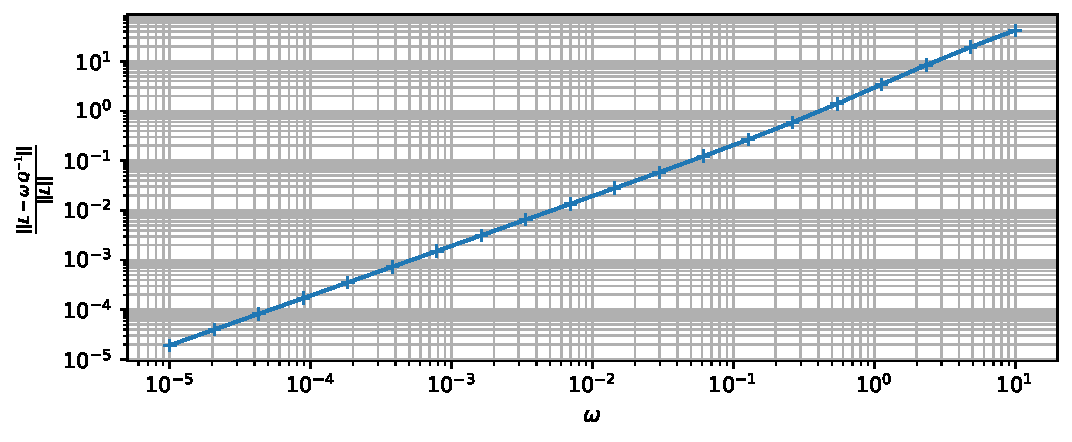
\includegraphics{./Hill_tensor_files/figure-pdf/fig-error-output-1.pdf}

}

\caption{\label{fig-error}Influence of the aspect ratio on the
contribution tensor}

\end{figure}



\end{document}
